\documentclass[a4paper]{article}

% Shared Preamble for MathLatexDocs

% --- Core Packages ---
\usepackage[english]{babel}
\usepackage[utf8]{inputenc}
\usepackage{amsmath}
\usepackage{amsthm}
\usepackage{amssymb}
\usepackage{mathtools}
\usepackage{graphicx}
\usepackage{microtype} % Better justification and fewer overfull hboxes
\usepackage{bm}
\usepackage{enumitem}
\usepackage{booktabs}
\usepackage{mathrsfs}

% --- Layout & Design ---
\usepackage{docmute}
\usepackage{subfiles} % Support for master/subfile structure
\usepackage[colorinlistoftodos]{todonotes}
\usepackage[colorlinks=true, linkcolor=blue, citecolor=magenta]{hyperref}
\usepackage{cleveref} % Better cross-referencing
\usepackage{tcolorbox} % For styled boxes
\usepackage{tikz} % For drawing diagrams
\usetikzlibrary{arrows.meta,positioning}

% --- Theorem Environments (Classic Style) ---
\makeatletter
\@ifundefined{classicthm}{%
  \newtheorem{classicthm}{Theorem}[section]
  \newtheorem{classicdef}[classicthm]{Definition}
  \newtheorem{classiclem}[classicthm]{Lemma}
  \newtheorem{theorem}{Theorem}[section]
  \newtheorem{corollary}{Corollary}[theorem]
  \newtheorem{lemma}[theorem]{Lemma}
  \newtheorem{definition}{Definition}[section]
  \newtheorem{proposition}[theorem]{Proposition}
  \newtheorem{remark}[theorem]{Remark}
  \newtheorem{example}[theorem]{Example}
}{}

% Wrappers to maintain compatibility with the {Title}{Label} syntax used in files
\@ifundefined{mytheorem}{%
  \newenvironment{mytheorem}[2]{%
    \begin{classicthm}[#1]\label{thm:#2}
  }{%
    \end{classicthm}
  }
  
  \newenvironment{mydefinition}[2]{%
    \begin{classicdef}[#1]\label{def:#2}
  }{%
    \end{classicdef}
  }
  
  \newenvironment{mylemma}[2]{%
    \begin{classiclem}[#1]\label{lem:#2}
  }{%
    \end{classiclem}
  }
}{}
\makeatother

% --- Custom Commands ---
\providecommand{\Z}{\mathbb{Z}}
\providecommand{\R}{\mathbb{R}}
\providecommand{\C}{\mathbb{C}}
\providecommand{\N}{\mathbb{N}}
\providecommand{\G}{\mathcal{G}}
\providecommand{\Lop}{\mathcal{L}}
\providecommand{\PP}{\mathcal{P}}
\providecommand{\dd}{\,\mathrm{d}}
\providecommand{\bitand}{\mathbin{\&}}
\providecommand{\CFDots}{\genfrac{}{}{0pt}{0}{}{\ddots}}


\title{\textbf{From Khinchin's Constant to the Gauss--Kuzmin--Wirsing Constant}\\[4pt]\large Continued Fractions, the Gauss Map, Invariant Measure, and Transfer-Operator Spectral Theory}
\author{Emil Kerimov}
\date{September 2026}
\begin{document}
\maketitle
\begin{abstract}
This note develops a self-contained path from the statistics of continued fractions to the Gauss measure and the spectral theory of the Gauss map. We begin with Khinchin's constant as motivation, then derive the Gauss map and its invariant probability measure, construct the Frobenius--Perron (transfer) operator, solve its invariant-density equation, explain the Gauss--Kuzmin theorem, and finally discuss the Gauss--Kuzmin--Wirsing constant as the magnitude of the dominant nontrivial spectral mode. Particular attention is paid to why the density $(1+x)^{-1}$ appears naturally and how the eigenvalue near $-0.303663$ can be approximated numerically.
\end{abstract}
\tableofcontents
\newpage

\section{Motivation: Khinchin's constant}
A positive irrational number has a simple continued-fraction expansion
\begin{equation}
 x=[a_0;a_1,a_2,a_3,\ldots]
 =a_0+\cfrac{1}{a_1+\cfrac{1}{a_2+\cfrac{1}{a_3+\ddots}}},
\end{equation}
where $a_0\in\mathbb Z$ and $a_n\in\N$ for $n\ge1$. For $x\in(0,1)$, $a_0=0$.

The partial quotients are highly non-uniform. For ``typical'' $x$, small values occur frequently but large values remain possible. Khinchin's theorem says something unexpectedly rigid: for Lebesgue-almost every irrational $x$, the geometric mean of the partial quotients converges to a universal constant,
\begin{equation}
 \lim_{N\to\infty}\left(a_1a_2\cdots a_N\right)^{1/N}=K_0,
\end{equation}
where
\begin{equation}
 K_0=\prod_{k=1}^{\infty} k^{\log_2\!\left(1+\frac{1}{k(k+2)}\right)}
 \approx 2.6854520010653064453\ldots.
\end{equation}
The surprising part is that the answer is the same for almost every real number even though individual continued fractions can look completely different.

The distribution behind Khinchin's theorem is the Gauss--Kuzmin distribution. Understanding it leads naturally to dynamical systems and ergodic theory.

\section{Continued fractions and the Gauss map}
For $x\in(0,1)$ irrational, define
\begin{equation}
 a_1=\left\lfloor\frac1x\right\rfloor,
 \qquad
 x_1=\frac1x-a_1.
\end{equation}
Repeating gives
\begin{equation}
 x_n=T^n(x),
 \qquad
 T(x)=\frac1x-\left\lfloor\frac1x\right\rfloor.
\end{equation}
The map $T:(0,1)\to(0,1)$ is the \emph{Gauss map}. If
\begin{equation}
 x=[0;a_1,a_2,a_3,\ldots],
\end{equation}
then
\begin{equation}
 T(x)=[0;a_2,a_3,a_4,\ldots].
\end{equation}
Thus applying $T$ shifts the continued-fraction sequence by one place.

For each $k\ge1$, define the branch interval
\begin{equation}
 I_k=\left(\frac1{k+1},\frac1k\right].
\end{equation}
On $I_k$,
\begin{equation}
 T(x)=\frac1x-k.
\end{equation}
Every branch maps bijectively onto $(0,1)$. Solving $T(x)=y$ on the $k$th branch gives the inverse branch
\begin{equation}
 \phi_k(y)=\frac1{k+y},
 \qquad
 \left|\phi_k'(y)\right|=\frac1{(k+y)^2}.
\end{equation}

\section{Invariant probability and the Gauss measure}
\begin{definition}
A probability measure $\mu$ on $(0,1)$ is \emph{invariant} under $T$ if
\begin{equation}
 \mu(T^{-1}A)=\mu(A)
\end{equation}
for every measurable set $A\subset(0,1)$.
\end{definition}
Invariance means that if $X$ is distributed according to $\mu$, then $T(X)$ has the same distribution. It does not mean that individual points are fixed.

The distinguished invariant probability measure is the \emph{Gauss measure}, whose density with respect to Lebesgue measure is
\begin{equation}
 h(x)=\frac{1}{\ln2}\frac1{1+x},
 \qquad 0<x<1.
\end{equation}
Normalization follows from
\begin{equation}
 \int_0^1\frac{\dd x}{1+x}=\ln2.
\end{equation}
Hence
\begin{equation}
 \mu(A)=\frac1{\ln2}\int_A\frac{\dd x}{1+x}.
\end{equation}

\subsection{Deriving the invariant-density equation}
Let $f$ be an arbitrary density and let $Y=T(X)$. For a fixed $y$, every inverse branch contributes probability from $x_k=\phi_k(y)=1/(k+y)$. The change-of-variables formula therefore gives
\begin{equation}
 (\PP f)(y)=\sum_{k=1}^{\infty}f\!\left(\frac1{k+y}\right)\frac1{(k+y)^2}.
 \label{gkw:eq:PF}
\end{equation}
The operator $\PP$ is the Frobenius--Perron, or transfer, operator of the Gauss map.

An invariant density is a fixed point:
\begin{equation}
 \PP f=f.
 \label{gkw:eq:fixed}
\end{equation}

\subsection{Why $1/(1+x)$ appears}
We now derive rather than guess the shape of the Gauss density. Suppose
\begin{equation}
 f(x)=\frac{C}{1+x}.
\end{equation}
Then
\begin{align}
 (\PP f)(y)
 &=C\sum_{k=1}^{\infty}
 \frac{1}{1+1/(k+y)}\frac1{(k+y)^2}\\
 &=C\sum_{k=1}^{\infty}
 \frac1{(k+y)(k+y+1)}\\
 &=C\sum_{k=1}^{\infty}
 \left(\frac1{k+y}-\frac1{k+y+1}\right)\\
 &=\frac{C}{1+y}.
\end{align}
The infinite sum telescopes. Thus every density of this shape is a fixed point up to normalization. Since
\begin{equation}
 1=\int_0^1f(x)\dd x=C\ln2,
\end{equation}
we obtain
\begin{equation}
 \boxed{h(x)=\frac1{\ln2(1+x)}}.
\end{equation}

There is a useful reverse-engineering argument. Put $t=k+y$. To obtain a telescoping term, seek
\begin{equation}
 f(1/t)\frac1{t^2}=g(t)-g(t+1).
\end{equation}
Choosing the simplest rational telescoper $g(t)=C/t$ yields
\begin{equation}
 f(1/t)\frac1{t^2}=\frac{C}{t(t+1)},
\end{equation}
and hence
\begin{equation}
 f(1/t)=\frac{Ct}{t+1}.
\end{equation}
With $t=1/x$ this becomes exactly $f(x)=C/(1+x)$.

\section{The Gauss--Kuzmin distribution}
The event that the first continued-fraction digit equals $k$ is
\begin{equation}
 \{a_1=k\}=\left(\frac1{k+1},\frac1k\right].
\end{equation}
Therefore its Gauss-measure probability is
\begin{align}
 p_k
 &=\mu(a_1=k)\\
 &=\frac1{\ln2}\int_{1/(k+1)}^{1/k}\frac{\dd x}{1+x}\\
 &=\frac1{\ln2}\ln\left(\frac{(k+1)^2}{k(k+2)}\right)\\
 &=\boxed{\log_2\left(1+\frac1{k(k+2)}\right)}.
\end{align}
The first few probabilities are approximately
\begin{center}
\begin{tabular}{c c}
\toprule
$k$ & $p_k$\\
\midrule
1 & $0.4150374993$\\
2 & $0.1699250014$\\
3 & $0.0931094044$\\
4 & $0.0588936891$\\
5 & $0.0406423630$\\
\bottomrule
\end{tabular}
\end{center}

The tail is asymptotically
\begin{equation}
 p_k=\log_2\left(1+\frac1{k(k+2)}\right)
 \sim\frac{1}{(\ln2)k^2}.
\end{equation}
This $k^{-2}$ tail explains why the arithmetic mean of $a_n$ diverges under the Gauss distribution, while suitable logarithmic averages remain finite.

\section{Khinchin's constant from the Gauss distribution}
The logarithm converts the geometric mean into an ordinary average:
\begin{equation}
 \frac1N\ln(a_1\cdots a_N)=\frac1N\sum_{n=1}^N\ln a_n.
\end{equation}
The Gauss map is ergodic with respect to Gauss measure. Thus, for suitable observables $g$,
\begin{equation}
 \frac1N\sum_{n=1}^N g(T^{n-1}x)
 \longrightarrow
 \int_0^1g(y)\,h(y)\dd y
\end{equation}
for $\mu$-almost every $x$.
Taking $g(y)=\ln\lfloor1/y\rfloor$ gives
\begin{align}
 \ln K_0
 &=\sum_{k=1}^{\infty}p_k\ln k\\
 &=\frac1{\ln2}\sum_{k=1}^{\infty}
 \ln k\,\ln\left(1+\frac1{k(k+2)}\right).
\end{align}
Exponentiating gives Khinchin's constant in the equivalent product form
\begin{equation}
 K_0=\prod_{k=1}^{\infty}k^{p_k}.
\end{equation}

\section{Gauss--Kuzmin theorem: convergence to equilibrium}
The invariant density is a stationary distribution, but the deeper statement is that the system forgets initial conditions.
If $f$ is an admissible initial density, then
\begin{equation}
 \PP^n f\longrightarrow h
\end{equation}
under suitable norms. Equivalently, the distribution of $T^n(x)$ approaches Gauss measure.

For continued-fraction digits, this says that for each fixed $k$,
\begin{equation}
 \Pr(a_{n+1}=k)\longrightarrow p_k
 =\log_2\left(1+\frac1{k(k+2)}\right).
\end{equation}
The theorem is a dynamical statement: iterating the map shifts the continued fraction, while the statistical law approaches the invariant law.

\section{The transfer operator as an infinite-dimensional matrix}
The transfer operator is linear:
\begin{equation}
 \PP(af+bg)=a\PP f+b\PP g.
\end{equation}
Thus the invariant-density equation is an eigenvalue problem,
\begin{equation}
 \PP f=\lambda f.
\end{equation}
The Gauss density is the eigenfunction for
\begin{equation}
 \lambda_0=1.
\end{equation}

A useful way to think about this is the finite-dimensional analogy. If a matrix $M$ has eigenpairs $(\lambda_j,v_j)$, then
\begin{equation}
 M^n v_j=\lambda_j^n v_j.
\end{equation}
The eigenvalue $1$ gives the stationary component. Eigenvalues with modulus less than $1$ give decaying modes.

For the Gauss transfer operator, the corresponding decomposition is schematically
\begin{equation}
 \PP^n f
 =h+C_1\lambda_1^n\phi_1+C_2\lambda_2^n\phi_2+\cdots,
\end{equation}
where $\lambda_1$ is the dominant nontrivial eigenvalue in the relevant spectral setting.

\section{Why a negative eigenvalue can occur}
Each inverse branch
\begin{equation}
 \phi_k(x)=\frac1{k+x}
\end{equation}
is orientation reversing because
\begin{equation}
 \phi_k'(x)=-\frac1{(k+x)^2}<0.
\end{equation}
This gives useful geometric intuition for oscillatory modes, although it does not by itself prove the sign of any particular eigenvalue. The sign and magnitude of the dominant nontrivial eigenvalue are global spectral properties of $\PP$.

If
\begin{equation}
 \PP\phi_1=\lambda_1\phi_1,
 \qquad \lambda_1<0,
\end{equation}
then
\begin{equation}
 \PP^n\phi_1=\lambda_1^n\phi_1.
\end{equation}
Thus the perturbation changes sign on every iteration while shrinking geometrically. This is the meaning of the alternating sign in the Gauss--Kuzmin asymptotics.

\section{The Gauss--Kuzmin--Wirsing constant}
The dominant nontrivial eigenvalue of the Gauss transfer operator is numerically
\begin{equation}
 \boxed{\lambda_1=-0.3036630028987326585974481219\ldots}
\end{equation}
(up to the convention/function-space details used to define the spectral problem). Its magnitude
\begin{equation}
 \boxed{\theta=0.3036630028987326585\ldots}
\end{equation}
is called the Gauss--Kuzmin--Wirsing constant.

The leading asymptotic form of convergence can be written schematically as
\begin{equation}
 \PP^n f-h
 \sim C_f(-\theta)^n\phi_1,
 \qquad n\to\infty,
\end{equation}
provided the initial density has a nonzero component in the corresponding eigendirection. Therefore the dominant error alternates in sign and has magnitude proportional to $\theta^n$.

For scale, 
\begin{equation}
\theta^2\approx0.09221,\quad
\theta^3\approx0.02801,\quad
\theta^4\approx0.00851,\quad
\theta^{10}\approx6.7\times10^{-6}.
\end{equation}
Thus the convergence is very rapid.

\section{How to calculate the constant numerically}
There is no comparably simple closed-form expression for $\theta$. It arises as the solution of an infinite-dimensional eigenvalue problem. A practical calculation replaces $\PP$ by a finite-dimensional approximation.

\subsection{Grid/collocation approximation}
Choose grid points
\begin{equation}
 0<x_1<\cdots<x_N<1
\end{equation}
and a finite-dimensional interpolation space. For a basis $\{\psi_j\}_{j=1}^N$, approximate
\begin{equation}
 f(x)\approx\sum_{j=1}^Nc_j\psi_j(x).
\end{equation}
Evaluate $\PP\psi_j$ at the grid points and construct the matrix
\begin{equation}
 M_{ij}\approx(\PP\psi_j)(x_i).
\end{equation}
Then solve
\begin{equation}
 M\bm c=\lambda\bm c.
\end{equation}
The eigenvalue near $1$ approximates the invariant density mode, while the dominant negative nontrivial eigenvalue approaches $-\theta$ as the approximation is refined, provided the discretization respects the regularity of the operator.

\subsection{Analytic-basis approach}
A more accurate approach uses the analytic structure of the inverse branches. Expand
\begin{equation}
 f(x)=\sum_{m\ge0}c_mx^m.
\end{equation}
Then
\begin{align}
 (\PP f)(x)
 &=\sum_{k=1}^{\infty}\frac1{(k+x)^2}
 \sum_{m\ge0}c_m\left(\frac1{k+x}\right)^m\\
 &=\sum_{m\ge0}c_m\sum_{k=1}^{\infty}\frac1{(k+x)^{m+2}}.
\end{align}
The inner sums are Hurwitz-zeta-type functions,
\begin{equation}
 \sum_{k=1}^{\infty}\frac1{(k+x)^s}=\zeta(s,1+x).
\end{equation}
One may therefore represent $\PP$ on a suitable analytic basis, truncate the resulting infinite matrix, and compute its eigenvalues. Increasing the truncation dimension gives convergent numerical approximations to isolated eigenvalues.

\subsection{Power-series coefficients and the invariant mode}
The invariant density can itself be expanded around $x=0$:
\begin{equation}
 \frac1{1+x}=1-x+x^2-x^3+\cdots,
 \qquad |x|<1.
\end{equation}
Thus the eigenvalue-$1$ eigenfunction is represented particularly simply in a power-series basis. The nontrivial eigenfunction associated with $-\theta$ is more complicated, but it can likewise be approximated by finite series or rational/analytic bases.

\section{A useful computational experiment}
A direct numerical experiment can be organized as follows.
\begin{enumerate}[label=\arabic*.]
\item Choose an initial density, for example $f_0(x)=1$.
\item Numerically evaluate
\begin{equation}
 f_{n+1}(x)=\sum_{k=1}^{K}\frac{f_n(1/(k+x))}{(k+x)^2}
\end{equation}
with $K$ sufficiently large and with interpolation in $x$.
\item Compare $f_n$ to the normalized Gauss density $h(x)$.
\item Measure an error such as
\begin{equation}
 E_n=\sup_{x\in[0,1]}|f_n(x)-h(x)|.
\end{equation}
\item After transients have decayed, inspect the ratio of signed errors in a fixed linear functional $\ell$:
\begin{equation}
 \frac{\ell(f_{n+1}-h)}{\ell(f_n-h)}.
\end{equation}
Generically this ratio approaches $-\theta$ when the dominant nontrivial mode is present.
\end{enumerate}
This is a particularly concrete way to see both the negative sign and the numerical value of the Gauss--Kuzmin--Wirsing constant.

\section{From transfer operators to deeper spectral theory}
The operator can be generalized to a parameter $s$ by
\begin{equation}
 (\Lop_s f)(x)=\sum_{n=1}^{\infty}\frac1{(n+x)^{2s}}
 f\left(\frac1{n+x}\right).
\end{equation}
At $s=1$, $\Lop_s$ becomes the Gauss transfer operator $\PP$.

This family is closely connected to dynamical zeta functions, Fredholm determinants, and the arithmetic of periodic orbits. Periodic points of the Gauss map correspond to periodic continued fractions and hence to quadratic irrationals. Spectral determinants of suitable transfer operators encode arithmetic information and provide a bridge toward zeta functions.

A standard perspective is therefore
\begin{equation}
\text{continued fractions}
\longrightarrow
\text{Gauss map}
\longrightarrow
\text{transfer operator}
\longrightarrow
\text{spectrum}
\longrightarrow
\text{arithmetic information}.
\end{equation}

\section{Summary of the main equations}
For reference, the central chain of formulas is
\begin{align}
 T(x)&=\frac1x-\left\lfloor\frac1x\right\rfloor,\\
 \phi_k(x)&=\frac1{k+x},\\
 |\phi_k'(x)|&=\frac1{(k+x)^2},\\
 (\PP f)(x)&=\sum_{k=1}^{\infty}\frac{f(1/(k+x))}{(k+x)^2},\\
 h(x)&=\frac1{\ln2(1+x)},\\
 \PP h&=h,\\
 p_k&=\mu(a_1=k)
 =\log_2\left(1+\frac1{k(k+2)}\right),\\
 K_0&=\prod_{k=1}^{\infty}k^{p_k}\approx2.6854520010653064,\\
 \lambda_0&=1,\\
 \lambda_1&\approx-0.3036630028987327,\\
 \theta&=|\lambda_1|\approx0.3036630028987327.
\end{align}

\section{Conceptual picture}
The entire story can be summarized as follows. Continued-fraction digits are generated by repeatedly applying the Gauss map. The map has infinitely many inverse branches, and the corresponding Jacobians determine a transfer operator. The special density $(1+x)^{-1}/\ln2$ is invariant because substitution into the operator creates a telescoping series. Ergodicity converts the invariant measure into almost-sure long-run statistics, producing the Gauss--Kuzmin distribution and Khinchin's constant. Spectral theory then explains the rate at which arbitrary initial distributions approach equilibrium: the eigenvalue $1$ represents the stationary mode, while the dominant nontrivial eigenvalue near $-0.303663$ represents an alternating, exponentially decaying mode.

\begin{center}
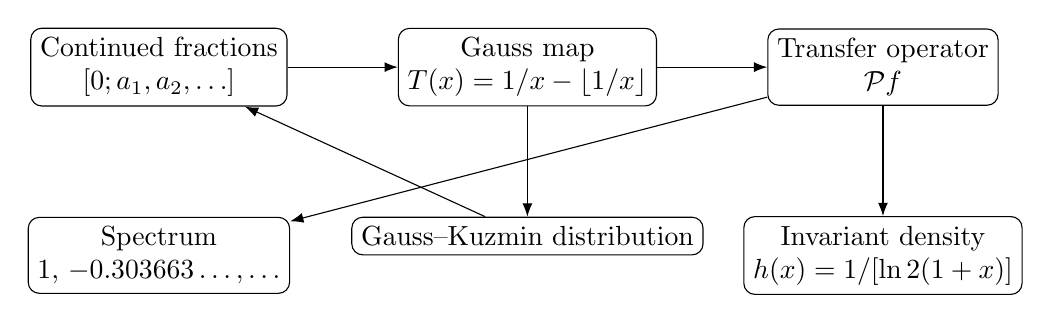
\begin{tikzpicture}[node distance=1.4cm, every node/.style={align=center}, >=Latex]
\node (cf) [draw, rounded corners] {Continued fractions\\$[0;a_1,a_2,\ldots]$};
\node (gm) [draw, rounded corners, right=of cf] {Gauss map\\$T(x)=1/x-\lfloor1/x\rfloor$};
\node (op) [draw, rounded corners, right=of gm] {Transfer operator\\$\PP f$};
\node (inv) [draw, rounded corners, below=of op] {Invariant density\\$h(x)=1/[\ln2(1+x)]$};
\node (dist) [draw, rounded corners, below=of gm] {Gauss--Kuzmin distribution};
\node (spec) [draw, rounded corners, below=of cf] {Spectrum\\$1,\,-0.303663\ldots,\ldots$};
\draw[->] (cf) -- (gm);
\draw[->] (gm) -- (op);
\draw[->] (op) -- (inv);
\draw[->] (gm) -- (dist);
\draw[->] (op) -- (spec);
\draw[->] (dist) -- (cf);
\end{tikzpicture}
\end{center}

\section*{Further directions}
Natural next topics include a proof of ergodicity of the Gauss map, the exact Gauss--Kuzmin error estimates, the function spaces on which the transfer operator has a discrete spectrum, explicit construction of the dominant nontrivial eigenfunction, Mayer's transfer operator, and the connection between dynamical zeta functions and the Riemann zeta function.

\end{document}
